% Authoritative, editable report. build_report.py updates tables, not this file.
% Compile here with: tectonic report.tex  (or pdflatex report.tex twice).
\documentclass[10pt,a4paper]{article}
\usepackage[T1]{fontenc}
\usepackage[utf8]{inputenc}
\usepackage[margin=21mm,headheight=14pt]{geometry}
\usepackage{newtxtext,newtxmath,microtype}
\usepackage{amsmath,booktabs,graphicx,xcolor,caption,subcaption,float}
\usepackage{fancyhdr,titlesec,enumitem,hyperref}
\definecolor{ink}{HTML}{193B50}
\definecolor{muted}{HTML}{526575}
\hypersetup{colorlinks=true,linkcolor=ink,urlcolor=ink,hypertexnames=false,pdftitle={Iterative solvers and domain decomposition for the Poisson equation},pdfauthor={}}
\graphicspath{{../results/}{figures/}}
\newcommand{\QsevenIterations}{17}
\newcommand{\QsevenResidual}{$7.586\times10^{-11}$}
\newcommand{\QsevenDifference}{$8.071\times10^{-11}$}
\newcommand{\QsevenSetup}{0.002563}
\newcommand{\QsevenSolve}{0.001712}
\newcommand{\BestP}{2}
\newcommand{\BestOverlap}{4}
\newcommand{\BestTime}{0.01115}
\setlength{\parindent}{0pt}
\setlength{\parskip}{5pt}
\setlength{\textfloatsep}{10pt}
\setlength{\intextsep}{8pt}
\captionsetup{font=small,labelfont=bf,skip=5pt}
\renewcommand{\arraystretch}{1.12}
\titleformat{\section}{\Large\bfseries\color{ink}}{}{0pt}{}
\titleformat{\subsection}{\normalsize\bfseries\color{ink}}{}{0pt}{}
\titlespacing*{\section}{0pt}{0pt}{9pt}
\titlespacing*{\subsection}{0pt}{9pt}{3pt}
\pagestyle{fancy}\fancyhf{}
\fancyhead[L]{\small\color{muted}WI4201\enspace /\enspace Computer project}
\fancyhead[R]{\small\color{muted}Poisson equation}
\fancyfoot[C]{\small\thepage}
\renewcommand{\headrulewidth}{0.3pt}
\newcommand{\norm}[1]{\left\lVert#1\right\rVert}
\newcommand{\Ah}{A_h}
\newcommand{\fh}{f_h}
\newcommand{\uh}{u_h}
\newcommand{\R}{\mathbb{R}}
\newcommand{\fig}[3]{\begin{figure}[H]\centering
  \includegraphics[width=#2\linewidth]{#1}\caption{#3}\end{figure}}
\begin{document}
\begin{titlepage}
\thispagestyle{empty}
\vspace*{18mm}
{\large\sffamily\color{muted}WI4201\quad ITERATIVE METHODS}\par
\vspace{15mm}
{\fontsize{34}{38}\selectfont\bfseries\color{ink}Solving the\\Poisson equation\par}
\vspace{9mm}
{\Large Finite differences, conjugate gradients\\and overlapping domain decomposition\par}
\vspace{13mm}
{\color{ink}\rule{\linewidth}{1pt}}\par
\vspace{7mm}
\begin{minipage}{.82\linewidth}
We compare stationary SSOR, conjugate gradient, and two preconditioned
variants on a common finite-difference problem. A manufactured solution
verifies spatial accuracy; residual histories and CPU measurements reveal
the trade-off between convergence and the cost of each iteration.
\end{minipage}
\vfill
{\small\color{muted}Pen-and-paper questions 1--6 and implementation questions 1--8.\\
Nameless working report. Numerical tables are generated from the experiment CSV files.}
\end{titlepage}
\setcounter{page}{1}

\section{Pen-and-paper analysis}
\subsection{1. Manufactured solution and boundary data}
On $\Omega=(0,1)^2$, the problem is $-\Delta u=f$ with $u=b$ on
$\partial\Omega$. For $u_{\mathrm{ex}}(x,y)=\sin(xy)$,
\[
 u_{xx}=-y^2\sin(xy),\qquad u_{yy}=-x^2\sin(xy),\qquad
 \boxed{f(x,y)=(x^2+y^2)\sin(xy).}
\]
The Dirichlet data are the restriction of the same function:
\[
 b(0,y)=b(x,0)=0,\qquad b(1,y)=\sin y,\qquad b(x,1)=\sin x.
\]
The values agree at all four corners.

\subsection{2. Matrix size, sparsity and bandwidth}
Divide each side into $N$ intervals, with $h=1/N$. Retaining boundary nodes
gives $n=(N+1)^2$ unknowns. We use $x$-fastest ordering:
\[
 (x_i,y_j)=(ih,jh),\qquad k=i+j(N+1),\qquad 0\leq i,j\leq N.
\]
At an interior node, the five-point approximation is
\begin{equation}
 (-\Delta_h u)_{i,j}=\frac{4u_{i,j}-u_{i-1,j}-u_{i+1,j}-u_{i,j-1}-u_{i,j+1}}{h^2}.
 \label{eq:stencil}
\end{equation}
Thus $\Ah\in\R^{n\times n}$ has nonzeros only on diagonal offsets
$0,\pm1,\pm(N+1)$ before boundary couplings are removed. Boundary rows
and columns become identity equations, so each interior row has at most
five nonzeros. For $N\geq2$,
\[
 \operatorname{nnz}(\Ah)=(N-1)^2+4(N-1)(N-2)+4N=5N^2-12N+9.
\]
Storage is $O(n)$. Both upper and lower bandwidths are $N+1$ for $N\geq3$.
For $N=1,2$, the final matrix is diagonal and the bandwidths are zero.

\subsection{3. A complete SSOR iteration}
Use the lecture convention $\Ah=D-E-F$, where $F=E^T$.
A forward sweep and a backward sweep together form one iteration:
\begin{align}
 (D-\omega E)u^{k+1/2}
  &=\omega\fh+\bigl[(1-\omega)D+\omega F\bigr]u^k,\\
 (D-\omega F)u^{k+1}
  &=\omega\fh+\bigl[(1-\omega)D+\omega E\bigr]u^{k+1/2}.
\end{align}
The interior Dirichlet Laplacian is symmetric positive definite (SPD), and
retaining a decoupled boundary identity block preserves this property.
SSOR therefore converges for $0<\omega<2$; we use $\omega=1.5$.
The code stores actual triangular entries $L=-E$, $U=-F$, so its factors
are written $D+\omega L$ and $D+\omega U$.

\clearpage
\section{Work estimates and preconditioning}
\subsection{4. Cost of SSOR}
Each sparse triangular solve and matrix--vector product uses $O(n)$
operations because the stencil has a bounded number of entries per row.
Vector updates and residual norms also cost $O(n)$. Hence one complete
SSOR iteration costs $O(n)$; $K$ iterations cost $O(Kn)$, using $O(n)$
storage. The iteration count is mesh dependent, so this is not a claim
of linear total solution cost.

\subsection{5(a). Conjugate gradient}
CG requires an SPD coefficient matrix. Initialise $u^0=0$,
$r^0=\fh$ and $p^0=r^0$. For $k=0,1,\ldots$, compute
\begin{align*}
 \alpha_k&=\frac{(r^k)^Tr^k}{(p^k)^T\Ah p^k}, &
 u^{k+1}&=u^k+\alpha_kp^k, &
 r^{k+1}&=r^k-\alpha_k\Ah p^k,\\
 \beta_k&=\frac{(r^{k+1})^Tr^{k+1}}{(r^k)^Tr^k}, &
 p^{k+1}&=r^{k+1}+\beta_kp^k.
\end{align*}
Every stopping test and convergence plot uses the recomputed residual
\begin{equation}
 \eta_k=\frac{\norm{\fh-\Ah u^k}_2}{\norm{\fh}_2}\leq10^{-10}.
 \label{eq:stop}
\end{equation}
The recurred $r^k$ is used only in the CG algebra, avoiding confusion
between the true residual and a preconditioned residual.

\subsection{5(b,c). SSOR-preconditioned CG}
The factored SSOR preconditioner is
\begin{equation}
 M_{\mathrm{SSOR}}=\frac{(D-\omega E)D^{-1}(D-\omega F)}{\omega(2-\omega)}.
 \label{eq:ssorM}
\end{equation}
The transpose factors, positive $D$, and positive scaling make $M$ SPD.
To apply $z=M^{-1}r$, solve $(D-\omega E)y=r$, solve
$(D-\omega F)v=Dy$, and set $z=\omega(2-\omega)v$.
PCG uses $\rho_k=(r^k)^Tz^k$, $p^0=z^0$,
$\alpha_k=\rho_k/[(p^k)^T\Ah p^k]$,
$\beta_k=\rho_{k+1}/\rho_k$, and $p^{k+1}=z^{k+1}+\beta_kp^k$.
Its two triangular solves are comparable to an SSOR sweep, with additional
matrix products, inner products and vector updates. Both methods cost
$O(n)$ per iteration, but their constants and iteration counts differ.

\subsection{6(a--d). One-level additive Schwarz}
$R_i$ restricts a global vector to subdomain $i$; $R_i^T$ inserts local
entries into a global vector, filling other positions with zero. The matrix
$A_i=R_i\Ah R_i^T$ is the principal submatrix associated with that set:
it describes a local correction with zero correction outside the set.
\[
 M_{\mathrm{AS}}^{-1}=\sum_{i=1}^pR_i^TA_i^{-1}R_i.
\]
Each $A_i$ is SPD. Because the index sets cover every unknown,
$v^TM_{\mathrm{AS}}^{-1}v=\sum_i(R_iv)^TA_i^{-1}(R_iv)>0$ for $v\ne0$.
Larger overlap generally improves exchange across interfaces but increases
local sizes, factorization cost and duplicated work. Local solves depend
only on the shared input residual and can run independently, followed by
accumulation. SSOR triangular solves instead have ordering dependencies.
Our implementation is serial; these are statements about potential parallelism.

\clearpage
\section{Implementation 1--2: discretization}
\subsection{1. Sparse assembly with boundary unknowns retained}
Let $m=N+1$, $T=\operatorname{tridiag}(-1,2,-1)$ and $I\in\R^{m\times m}$.
The preliminary operator is assembled using Kronecker products:
\[
 A_0=\frac{I\otimes T+T\otimes I}{h^2}.
\]
Let $P$ be diagonal with ones at interior points and zeros on the boundary,
and $B=I_n-P$. Let $g$ contain prescribed boundary values and zeros inside.
For the source vector $s_k=f(x_k,y_k)$, symmetric boundary handling gives
\begin{equation}
 \boxed{\Ah=PA_0P+B,\qquad \fh=P(s-A_0g)+g.}
\end{equation}
Both boundary rows and columns are removed before adding identity equations;
changing rows alone would destroy symmetry. The term $-A_0g$ moves known
boundary contributions to the interior right-hand side. Matrices use CSR
storage; Schwarz factorization inputs use CSC.

\subsection{2. Verification of second-order accuracy}
For $h=2^{-q}$, $q=3,\ldots,7$, a sparse direct solve gives $\uh$.
We compare with the exact solution sampled at the same nodes:
\[
 E_h=\norm{\uh-u_{\mathrm{ex}}^h}_\infty,\qquad
 p_{\mathrm{obs}}=\frac{\log(E_{2h}/E_h)}{\log2}.
\]
\begin{table}[H]\centering
\begin{tabular}{rrrrr}
\toprule
$N$ & $n$ & $h$ & $E_h$ & Order \\
\midrule
8 & 81 & $1/8$ & $1.313\times10^{-5}$ & -- \\
16 & 289 & $1/16$ & $3.444\times10^{-6}$ & 1.9313 \\
32 & 1089 & $1/32$ & $8.714\times10^{-7}$ & 1.9826 \\
64 & 4225 & $1/64$ & $2.185\times10^{-7}$ & 1.9956 \\
128 & 16641 & $1/128$ & $5.467\times10^{-8}$ & 1.9989 \\
\bottomrule
\end{tabular}

\caption{Maximum nodal error of the direct discrete solution. The order
approaches two as the mesh is refined.}\end{table}
\fig{discretization_error.png}{.77}{Discretization error versus grid spacing.
The dashed line has slope two; the measured points approach it.}
The fitted log--log slope over all five meshes is $1.9795$; the finest-pair
order is $1.9989$. Halving $h$ therefore reduces the error by approximately
four. This experiment measures spatial discretization error, independently
of iterative convergence.

\clearpage
\section{Implementation 3--5: stationary SSOR}
\subsection{3. Convergence histories}
We use $N=8,16,32,64$, $u^0=0$, $\omega=1.5$, and criterion~\eqref{eq:stop}.
One iteration is one forward--backward sweep. Figure~\ref{fig:ssor}
shows the true relative residual; refinement markedly slows convergence.
\begin{figure}[H]\centering
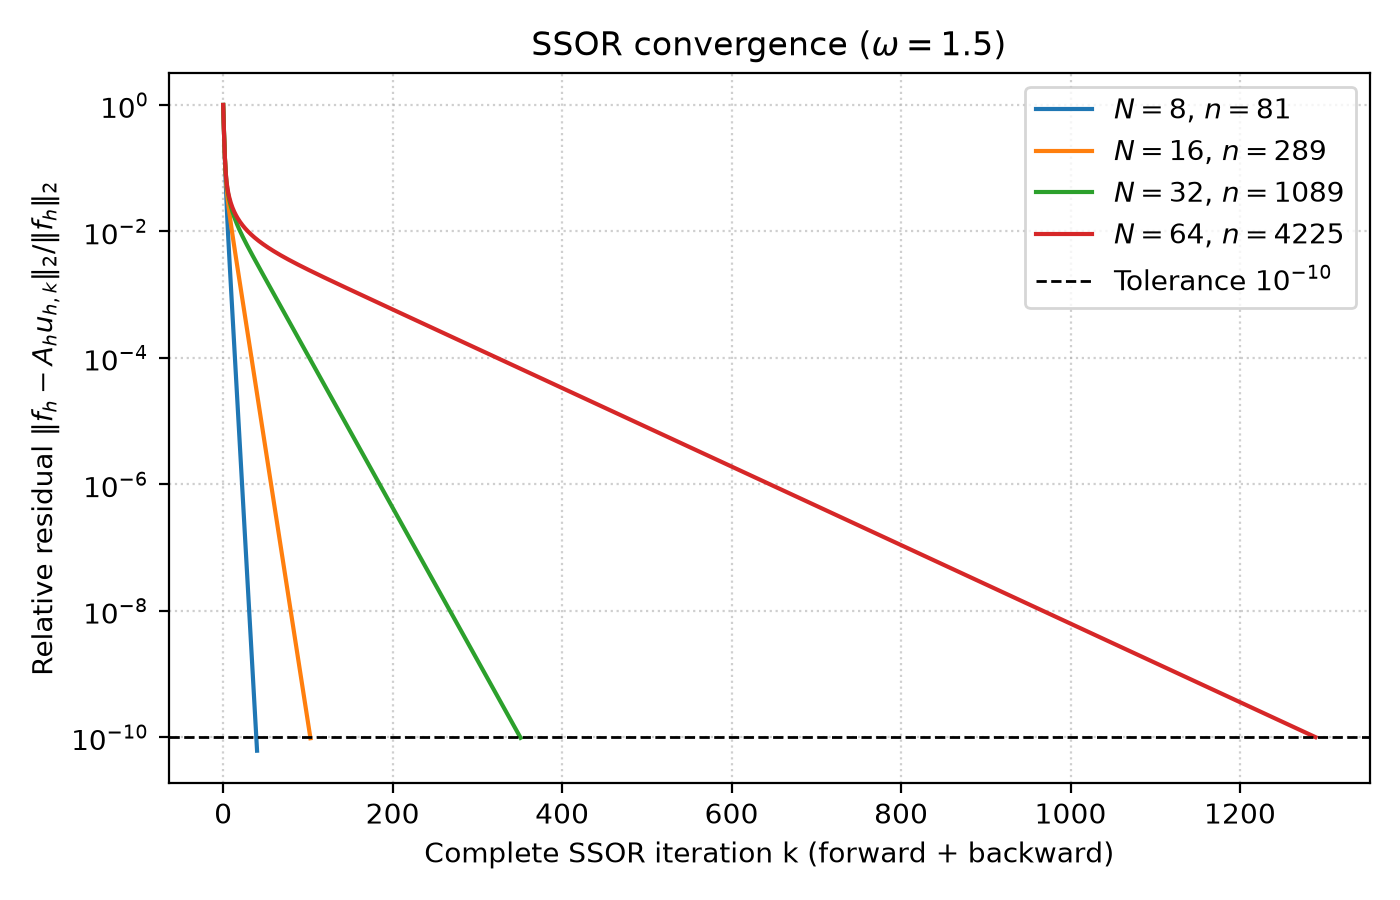
\includegraphics[width=.76\linewidth]{ssor_convergence.png}
\caption{SSOR convergence on four meshes. The late-stage decay becomes
shallower as $N$ increases.}\label{fig:ssor}\end{figure}
\subsection{4. Asymptotic residual reduction}
Define $q_k=\norm{r^k}_2/\norm{r^{k-1}}_2$ and estimate the asymptotic
factor by the geometric mean of the last five ratios:
$\widehat\rho=(\prod_{j=K-4}^{K}q_j)^{1/5}$.
\begin{table}[H]\centering\small
\begin{tabular}{rrrrrrr}
\toprule
$N$ & $q_{K-4}$ & $q_{K-3}$ & $q_{K-2}$ & $q_{K-1}$ & $q_K$ & $\widehat\rho$ \\
\midrule
8 & 0.577942 & 0.577926 & 0.577912 & 0.577900 & 0.577889 & 0.577914 \\
16 & 0.819473 & 0.819473 & 0.819473 & 0.819473 & 0.819473 & 0.819473 \\
32 & 0.946003 & 0.946002 & 0.946003 & 0.946002 & 0.946003 & 0.946002 \\
64 & 0.985798 & 0.985798 & 0.985798 & 0.985798 & 0.985798 & 0.985798 \\
\bottomrule
\end{tabular}

\caption{Final five complete-sweep residual reduction factors.}\end{table}
The ratios are nearly constant near convergence. Their mean rises from
$0.578$ to $0.986$, so SSOR removes a smaller fraction of the remaining
residual per sweep on finer grids.
\subsection{5. CPU time and the sparse-work estimate}
\begin{table}[H]\centering
\begin{tabular}{rrrrr}
\toprule
$N$ & $n$ & $K$ & CPU (s) & CPU$/nK$ \\
\midrule
8 & 81 & 40 & 0.02043 & $6.306\times10^{-6}$ \\
16 & 289 & 103 & 0.05312 & $1.785\times10^{-6}$ \\
32 & 1089 & 351 & 0.22656 & $5.927\times10^{-7}$ \\
64 & 4225 & 1289 & 1.40625 & $2.582\times10^{-7}$ \\
\bottomrule
\end{tabular}

\caption{SSOR iteration cost, excluding assembly and splitting/setup.}\end{table}
Time increases with both $n$ and $K$, as expected from $O(nK)$ sparse work.
The falling normalized cost suggests that fixed library-call overhead matters
more on small grids. These measurements do not establish an asymptotic CPU
scaling law. CPU measurements use repeated short solves;
the full timing protocol is given on page~8.

\clearpage
\section{Implementation 6: CG and SSOR-PCG}
The same four meshes, zero initial guesses and true-residual tolerance are
used for all methods. SSOR-PCG uses $\omega=1.5$ and constructs its factors
before timing. Direct-solution differences are recorded in
\texttt{cg\_summary.csv}; the largest across these runs is below $4\times10^{-9}$.
\begin{table}[H]\centering\small
\begin{tabular}{rlrrr}
\toprule
$N$ & Method & $K$ & CPU (s) & True residual \\
\midrule
8 & SSOR & 40 & 0.019231 & $6.091\times10^{-11}$ \\
8 & CG & 26 & 0.000423 & $9.500\times10^{-16}$ \\
8 & SSOR-PCG & 13 & 0.006250 & $6.978\times10^{-11}$ \\
16 & SSOR & 103 & 0.050000 & $9.596\times10^{-11}$ \\
16 & CG & 63 & 0.001225 & $9.647\times10^{-11}$ \\
16 & SSOR-PCG & 18 & 0.008621 & $3.676\times10^{-11}$ \\
32 & SSOR & 351 & 0.250000 & $9.746\times10^{-11}$ \\
32 & CG & 130 & 0.003012 & $6.851\times10^{-11}$ \\
32 & SSOR-PCG & 27 & 0.017857 & $7.596\times10^{-11}$ \\
64 & SSOR & 1289 & 1.406250 & $9.992\times10^{-11}$ \\
64 & CG & 259 & 0.013158 & $8.886\times10^{-11}$ \\
64 & SSOR-PCG & 48 & 0.056250 & $8.331\times10^{-11}$ \\
\bottomrule
\end{tabular}

\caption{Convergence and iteration-only CPU time. SSOR timings are repeated
here in the controlled method-comparison experiment.}\end{table}
\fig{cg_comparison.png}{.91}{True relative residuals for SSOR, CG and SSOR-PCG.
Each panel uses the same problem for all three methods.}
\textbf{Convergence.} SSOR-PCG uses the fewest iterations, and both CG
variants improve substantially on stationary SSOR. On the finer meshes,
doubling $N$ approximately doubles unpreconditioned CG's iteration count,
consistent with worsening conditioning under refinement. SSOR-PCG also
remains mesh dependent, although its iteration counts grow more slowly.

\textbf{CPU performance.} CG is faster than SSOR-PCG on all tested meshes.
The smaller PCG iteration count does not offset the cost of two SciPy
triangular solves per iteration. All methods perform $O(n)$ sparse work
per iteration; total cost depends on both $K$ and implementation constants.

\clearpage
\section{Implementation 7: additive Schwarz}
\subsection{Ownership rule and overlapping index sets}
Let $w=N/p$. Zero-based strip $s$ owns columns
$sw,\ldots,(s+1)w-1$, with column $N$ added to the final strip.
Internal interface columns belong to the strip on the \emph{right}.
All $y$ rows are included, including physical boundary unknowns.
The owned range $[a_s,b_s]$ is extended to
\[
 [\max(0,a_s-\ell),\ \min(N,b_s+\ell)],\qquad \delta=\ell h.
\]
Thus $\ell=0$ gives disjoint sets covering every unknown exactly once;
$\delta$ is the one-sided extension, not the total intersection width.

\subsection{Setup once; apply repeatedly}
Setup constructs the index sets, extracts each principal submatrix, and
computes a sparse LU factorization with \texttt{splu}. These objects are
retained throughout PCG. Each application performs
\[
 r_i=R_ir,\qquad A_i z_i=r_i,\qquad z=\sum_{i=1}^{p}R_i^Tz_i.
\]
The factorizations are reused; no explicit inverse is formed. Corrections
at overlapping nodes are added without averaging, matching the prescribed
additive Schwarz formula.

\subsection{Verification against a direct solve}
Use $N=32$, $n=1089$, $p=4$, $\ell=2$ and $\delta=1/16$.
AS-PCG converges in \QsevenIterations\ iterations, with true relative
residual \QsevenResidual\ and maximum difference from the direct discrete
solution \QsevenDifference. Measured setup and iteration CPU times are
\QsevenSetup\,s and \QsevenSolve\,s, respectively.
\fig{schwarz_q7_convergence.png}{.77}{Verification run for AS-PCG.
The stopping test uses the true, unpreconditioned residual.}
Automated checks cover exact zero-overlap ownership, overlap coverage,
principal-submatrix extraction, invalid partitions and the single-subdomain
limit, in which the preconditioner applies the global direct inverse.
The numerical agreement verifies the \emph{discrete} solution; the spatial
error assessed in implementation question~2 is a separate quantity.

\clearpage
\section{Implementation 8: subdomains and overlap}
Fix $N=64$, $h=1/64$ and $n=4225$. We use $p=2,4,8,16$ (all divisors of
$N$), and $\ell=0,1,2,4$. All 16 AS-PCG runs satisfy~\eqref{eq:stop} and
agree with a sparse direct reference to within $10^{-7}$ in maximum norm.
\begin{table}[H]\centering\small\setlength{\tabcolsep}{5pt}
\begin{tabular}{rrrrrrrr}
\toprule
$p$ & $\ell$ & $\delta$ & $K$ & Setup (s) & PCG (s) & Total (s) & $n_{\max}$ \\
\midrule
2 & 0 & 0.000000 & 38 & 0.00732 & 0.01136 & 0.01869 & 2145 \\
2 & 1 & 0.015625 & 23 & 0.00635 & 0.00735 & 0.01370 & 2210 \\
2 & 2 & 0.031250 & 18 & 0.00684 & 0.00556 & 0.01239 & 2275 \\
2 & 4 & 0.062500 & 13 & 0.00684 & 0.00431 & 0.01115 & 2405 \\
4 & 0 & 0.000000 & 55 & 0.00586 & 0.01389 & 0.01975 & 1105 \\
4 & 1 & 0.015625 & 32 & 0.00684 & 0.00962 & 0.01645 & 1170 \\
4 & 2 & 0.031250 & 25 & 0.00781 & 0.00758 & 0.01539 & 1300 \\
4 & 4 & 0.062500 & 18 & 0.00830 & 0.00676 & 0.01506 & 1560 \\
8 & 0 & 0.000000 & 67 & 0.00488 & 0.01562 & 0.02051 & 585 \\
8 & 1 & 0.015625 & 40 & 0.00586 & 0.01087 & 0.01673 & 650 \\
8 & 2 & 0.031250 & 31 & 0.00781 & 0.01136 & 0.01918 & 780 \\
8 & 4 & 0.062500 & 29 & 0.01074 & 0.01190 & 0.02265 & 1040 \\
16 & 0 & 0.000000 & 91 & 0.00488 & 0.02273 & 0.02761 & 325 \\
16 & 1 & 0.015625 & 55 & 0.00684 & 0.01667 & 0.02350 & 390 \\
16 & 2 & 0.031250 & 45 & 0.00977 & 0.01923 & 0.02900 & 520 \\
16 & 4 & 0.062500 & 30 & 0.01562 & 0.02083 & 0.03646 & 780 \\
\bottomrule
\end{tabular}

\caption{Fixed-mesh parameter study. Setup includes index construction,
matrix extraction and factorization. PCG time excludes setup. Total is their
sum for one right-hand side; $n_{\max}$ is the largest local problem size.}
\end{table}
\subsection{8(a). Increasing overlap}
Every tested decomposition needs fewer iterations as overlap increases.
For example, at $p=4$, $K$ falls from $55$ at $\ell=0$ to $18$ at $\ell=4$.
The larger local corrections transfer information more effectively across
strip interfaces.
\subsection{8(b). Increasing the number of subdomains}
For fixed $h$ and $\ell=2$, increasing $p$ from $2$ to $16$ raises $K$
from $18$ to $45$. Smaller subdomains provide less global correction,
and this one-level method has no coarse solve to propagate long-range
error efficiently. This is a fixed-mesh observation rather than a
mesh-independent scalability result.
\fig{schwarz_q8_iterations.png}{.72}{Effect of overlap on the AS-PCG
iteration count for each fixed strip count.}

\clearpage
\section{Implementation 8: performance trade-offs}
\subsection{8(c). Local cost versus convergence}
Overlap increases duplicated work and local factorization sizes. At $p=4$,
$n_{\max}$ grows from $1105$ to $1560$ as $\ell$ rises from $0$ to $4$.
Fewer iterations therefore compete with more expensive setup and local
solves. In this run the lowest setup-plus-solve time is
\BestTime\,s at $p=\BestP$, $\ell=\BestOverlap$.
This is not a universal optimum: short CPU measurements vary with load,
caching, sparse ordering and timer resolution. Setup can be amortized
when solving multiple right-hand sides with the same matrix.
\begin{figure}[H]\centering
\begin{subfigure}{.49\linewidth}\centering
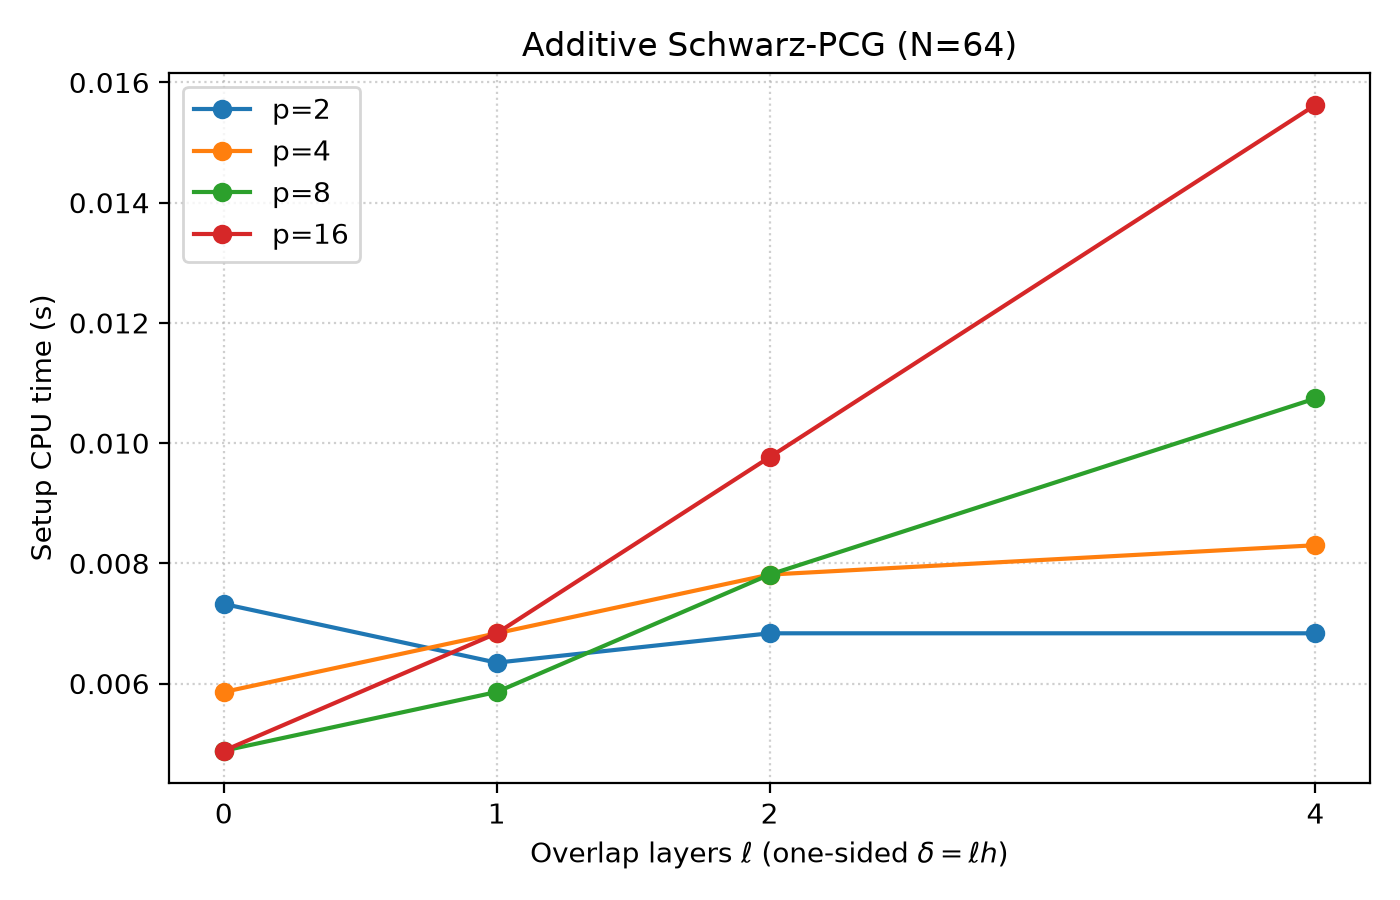
\includegraphics[width=\linewidth]{schwarz_q8_setup_time.png}
\caption{Setup cost.}\end{subfigure}\hfill
\begin{subfigure}{.49\linewidth}\centering
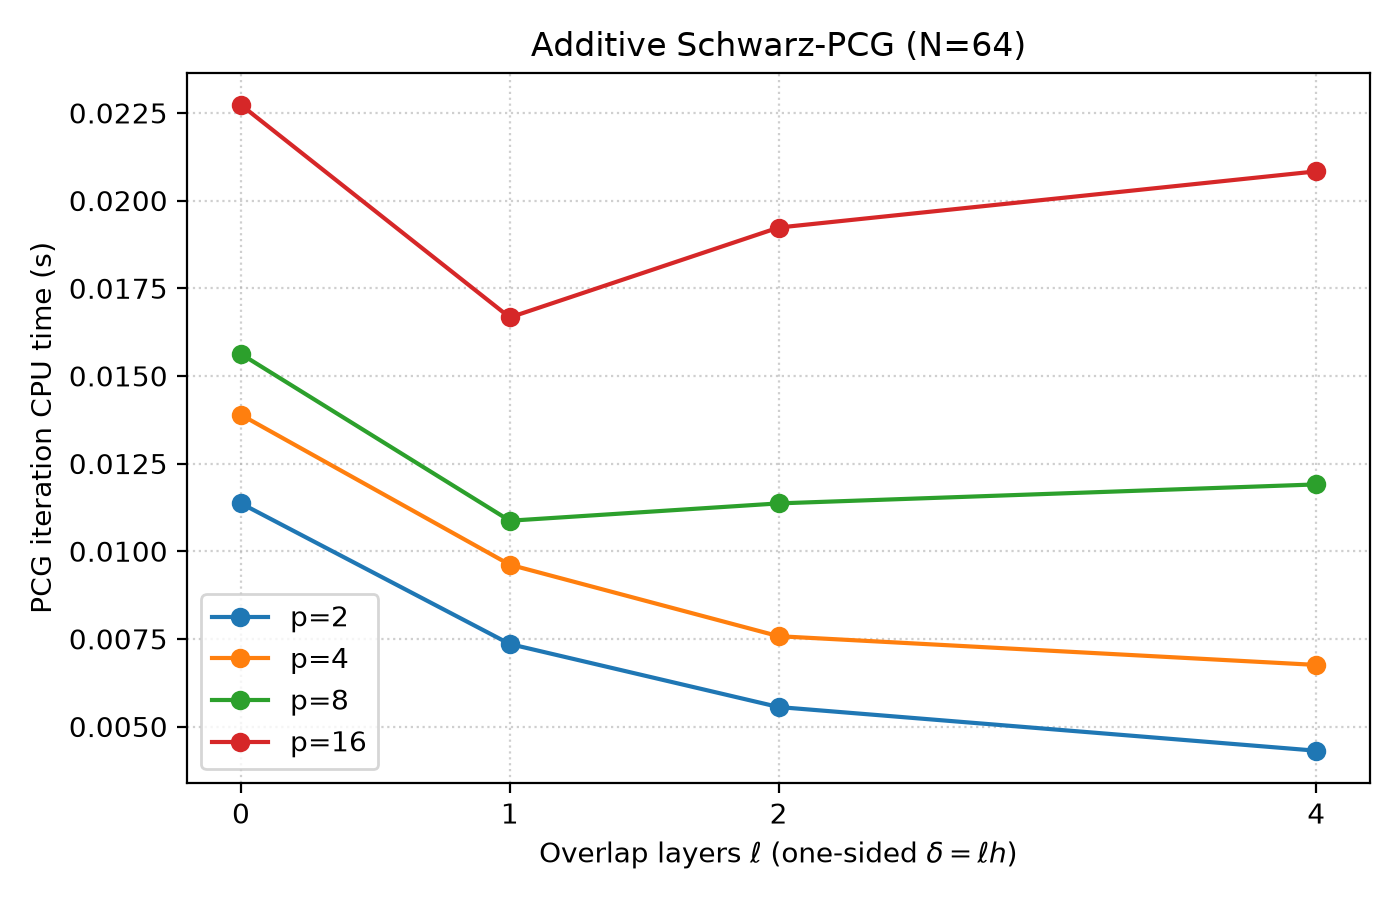
\includegraphics[width=\linewidth]{schwarz_q8_pcg_time.png}
\caption{Iteration-only cost.}\end{subfigure}
\caption{Separate costs explain why the overlap giving the fewest
iterations need not give the shortest total runtime.}\end{figure}
\subsection{8(d). Fixed-size method comparison}
For $N=64$, SSOR-PCG uses $\omega=1.5$; AS-PCG uses $p=4$, $\ell=2$.
\begin{table}[H]\centering
\begin{tabular}{lrrr}
\toprule
Method & $K$ & CPU (s) & True residual \\
\midrule
CG & 259 & 0.013889 & $8.886\times10^{-11}$ \\
SSOR-PCG & 48 & 0.056250 & $8.331\times10^{-11}$ \\
AS-PCG & 25 & 0.010417 & $3.837\times10^{-11}$ \\
\bottomrule
\end{tabular}

\caption{Method comparison excluding preconditioner setup.}\end{table}
AS-PCG takes the fewest iterations and is fastest in this comparison.
SSOR-PCG reduces iterations relative to CG but is slower in CPU time.
These rankings describe this serial implementation and these parameters.

\subsection{Timing protocol and reproducibility}
All CPU measurements use \texttt{time.process\_time}. Iteration timers
include preconditioner applications and true-residual checks, but exclude
assembly, splitting and preconditioner construction. Repeated solves
accumulate at least $0.25$ CPU seconds (cap $5000$ runs). Batched Schwarz
setup uses at least $0.25$ CPU seconds for question~7 and $0.15$ for
question~8 (cap $4096$ repetitions per batch).
The algorithms, boundary handling and domain decomposition are implemented
in project code; NumPy supplies array operations, SciPy supplies sparse
construction and direct/triangular solves, and Matplotlib supplies plots.
The README lists exact commands; \texttt{results/environment.json} records
software versions. No parallel implementation or measured speedup is claimed.
\end{document}
